\documentclass[12pt,a5]{bxjsarticle}

\usepackage{xltxtra}
\setmainfont{IPAPMincho}
\setsansfont{IPAPGothic}
\setmonofont{IPAGothic}
\XeTeXlinebreaklocale "ja"

\usepackage{hyperref}
\usepackage{listings}
\usepackage{verbatim}

\newcommand{\e}{\mathrm{e}}

\title{物理学情報処理論2 problem2}
\date{}

\begin{document}
\maketitle

$ \frac{d^2x}{dt^2} = - \frac{x}{r^3},
  \frac{d^2y}{dt^2} = - \frac{y}{r^3},
  r = \sqrt{x^2 + y^2},
  x(0) = 1,
  y(0) = 0,
  \frac{dx}{dt}(0) = 0,
  \frac{dy}{dt}(0) = 1
$
を、Euler法、Runge-Kutta法(2次、4次)、1次symplectic法を用いて解き、
plotしたものは以下のようになる。
比較すると、Euler法はかなり誤差が大きくなってしまっているが、
RK 2次の時点でかなり精度が良くなっている。
symplectic法はEuler法とほぼ同じ時間発展をするにも関わらず、
RK法程度まで精度が向上している。

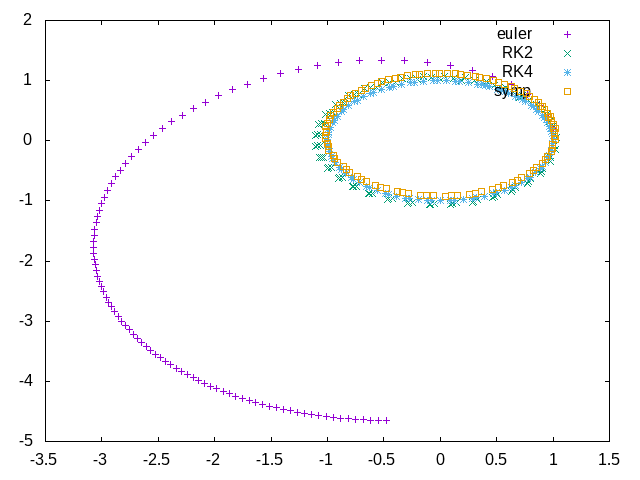
\includegraphics[width=\linewidth]{orbit.png}

今回のプログラムは、以下のようにコンパイルする。
\begin{lstlisting}[language=bash]
  $ g++ problem2.cpp
\end{lstlisting}

以下のスクリプトを用いて、orbit.datから図を生成した。
\lstinputlisting[caption=plot.sh,language=bash]{plot.sh}

\end{document}
